\section{Introduction}
\subsection{Motivation and Background}
Since the Fortran 2008 standard was published in 2010~\cite{iso2010fortran}, a handful of studies in the open literature
have provided encouraging assessments of Fortran's intrinsic parallel programming model, \gls{caf}, running in research
applications running at scale~\cite{preissl2011multithreaded,garain2015comparing,mozdzynski2015partitioned}.   One of the
most attractive features of \gls{caf} is the ability to express parallel algorithms once within the confines of a single
language standard without embedding the use of compiler directives or communication layers defined outside the Fortran
Fortran language standard (e.g., no \gls{mpi} or OpenMP.  In theory, this should leave the choice of communication layers
as a link-time decision.  Ideally, an application developer writes a standard Fortran-only application, compiles it with any
standard-conforming compiler, and possibly reserves the option to incorporate any one (or more) of several communication layers
at link-time.

Such flexibility poses the computing equivalent of what food author Michael Pollen termed ``The Omnivore's Dilemma:'' if I
belong to a species that owes some of its evolutionary advantage to being able to eat a wide variety of foods, what food is
best for me to eat?  Similarly, if I can express my parallel algorithm once using \gls{caf} and then consume cycles atop a
multitude of software stacks and hardware platforms, where best to consume cycles and using which supporting software stack?
Here we report the results of an initial study of the current options for compiling, linking, and executing a \gls{mini-app}
designed to be representative of the parallel numerical algorithms and physics employed in the \gls{icar} being developed at
the \gls{ncar}.

\gls{icar} simulates the motion of the atmosphere at kilometer length scales and produces flow patterns with a fidelity that is
attractive to the hydrology community, which studies surface water.  The animation in Figure~\ref{figure:icar} depicts atmospheric processes over North America.

\begin{figure}
   \vspace{-18pt}
   % Animate frames at 7 fps created via 'ffmpeg -i qvmovie.mp4 -r 7 frame%d.pngr', add control buttons,
   % and automatically play when the page is viewed:
   \vbox{\hspace{-24pt}
   \animategraphics[width=1.1\columnwidth,controls,autoplay]{7}{figures/icar/frames/frame}{1}{30}
   }
   \caption{An animation of atmospheric flow of water vapor (blues) and resulting precipitation (green to red) simulated by the \href{https://github.com/gutmann/icar}{\gls{icar}}.
\label{figure:icar}}
\end{figure}

\begin{figure*}
  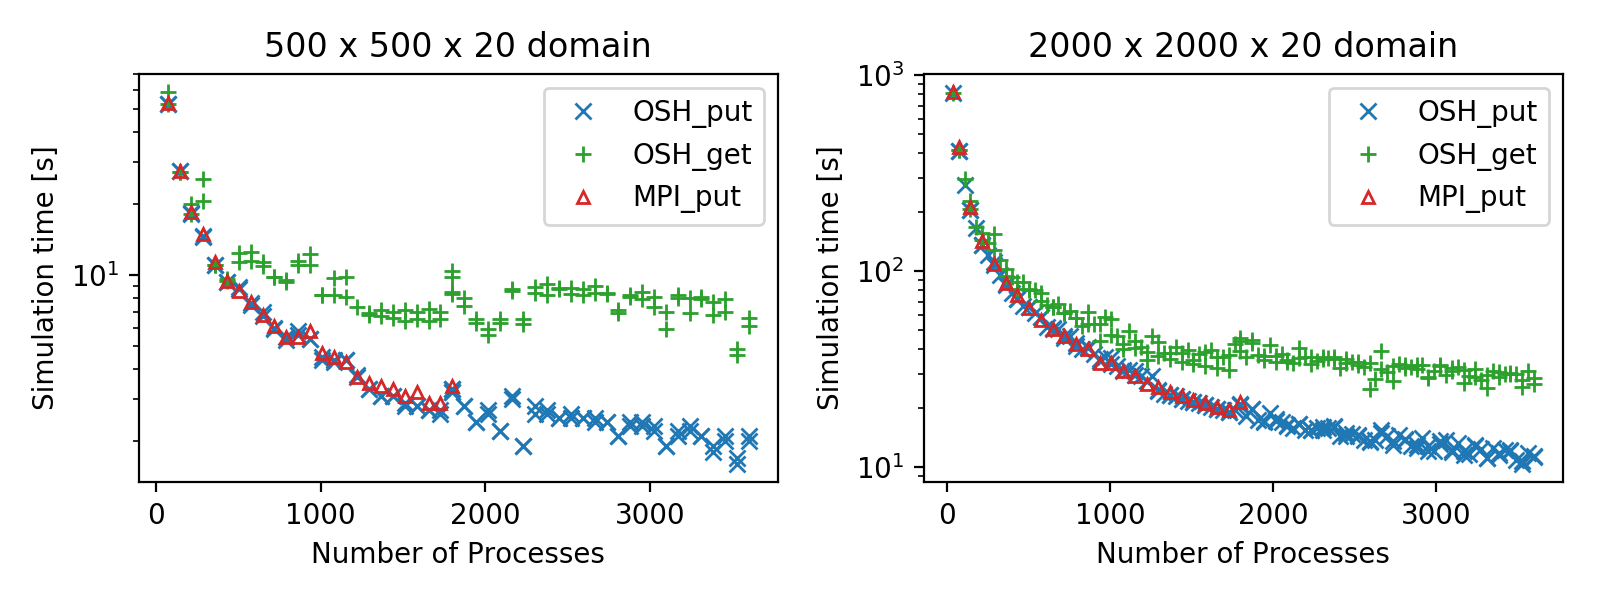
\includegraphics[width=\textwidth]{figures/fig1_speedup.png}
  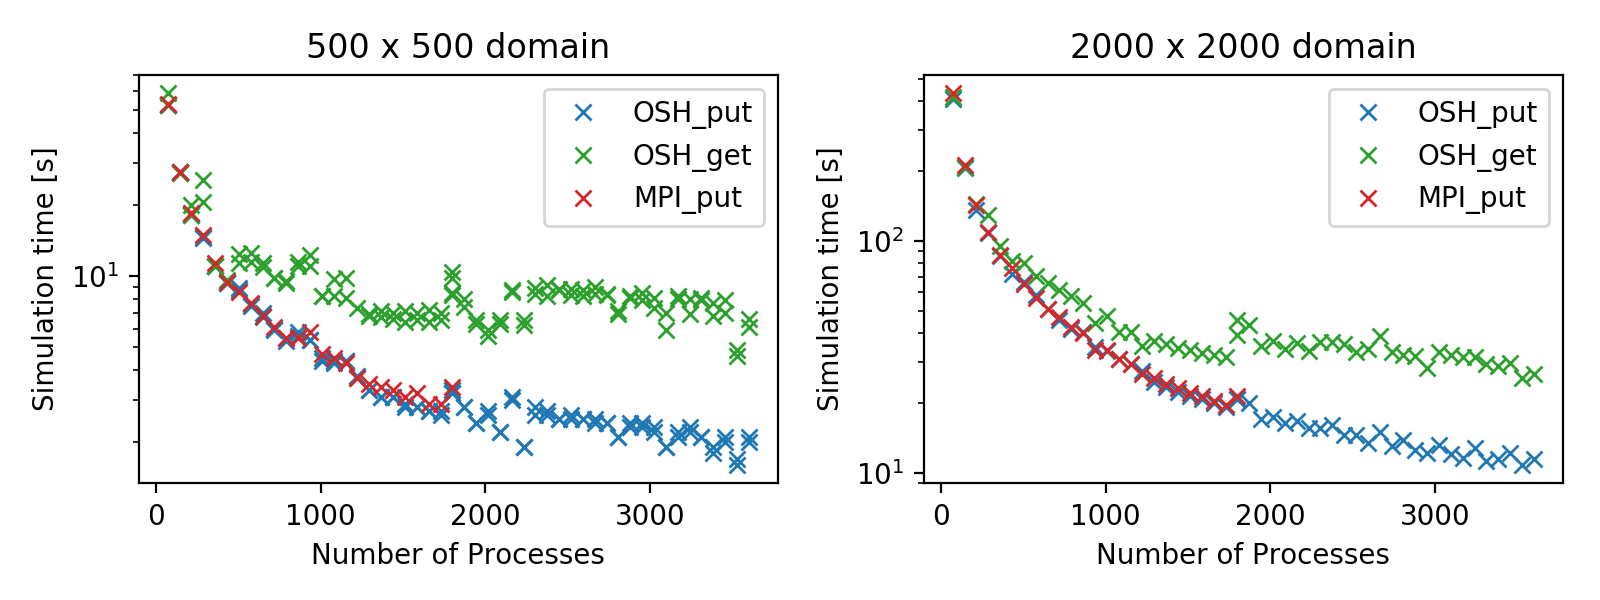
\includegraphics[width=\textwidth]{figures/fig2_timing.png}
  \caption{Speedup and timing results for two different domain sizes, two different communications backends (OSH=OpenSHMEM, MPI=MPI) and two different communication methods (``get'' and ``put'') using \href{https://github.com/gutmann/coarray_icar}{Coarray ICAR}.\label{fig1-2}}
\end{figure*}

\begin{figure*}
  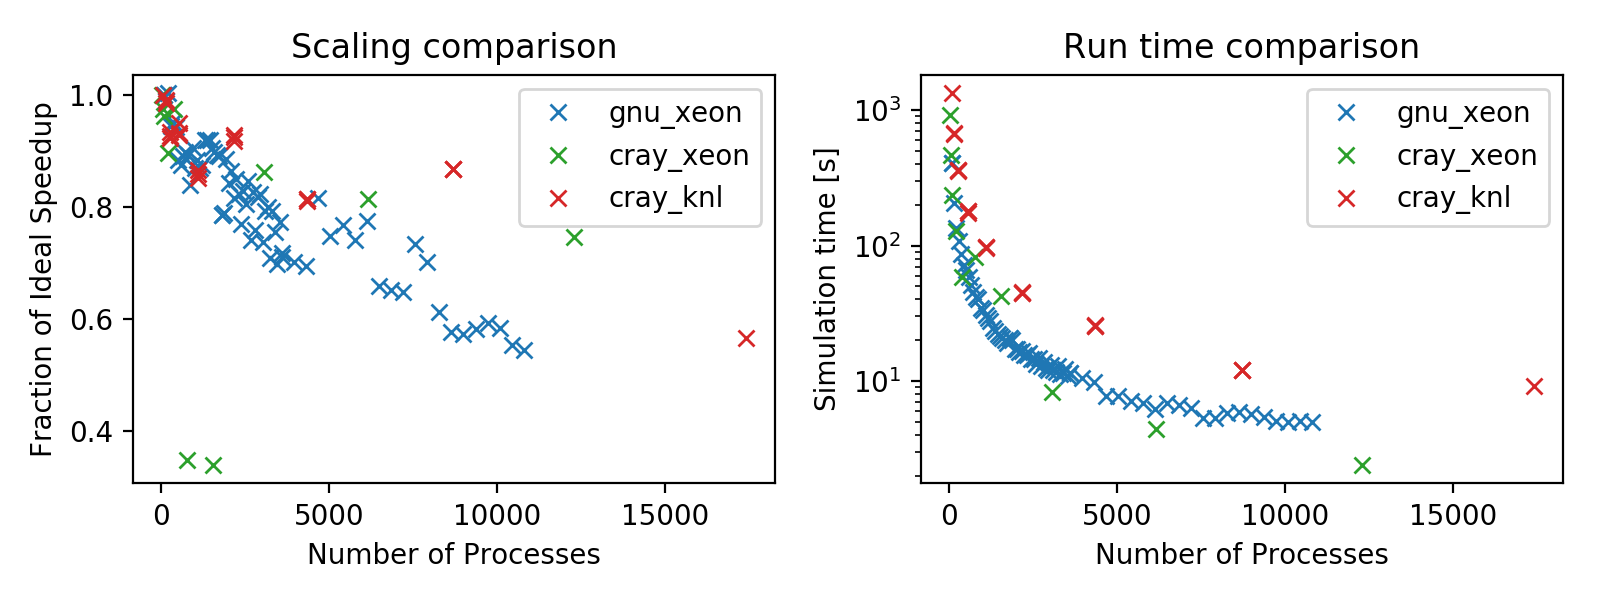
\includegraphics[width=\textwidth]{figures/fig3_cross_platform.png}
  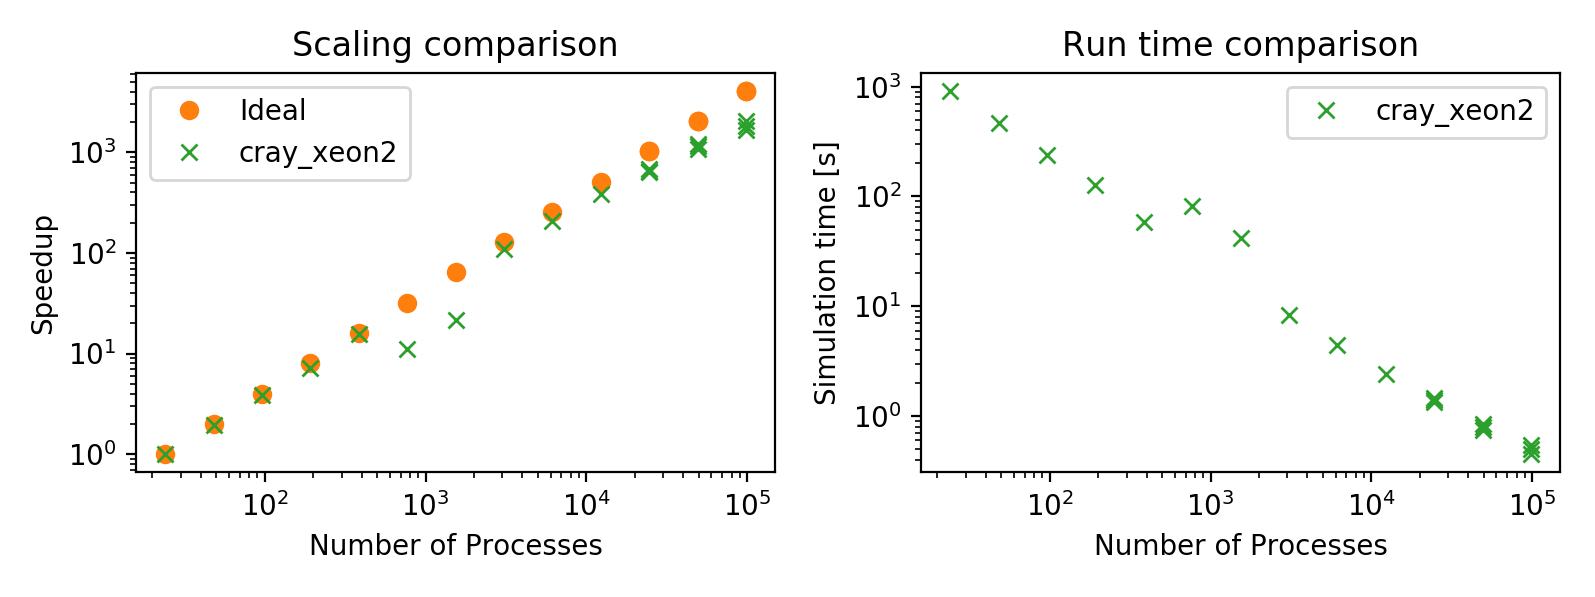
\includegraphics[width=\textwidth]{figures/fig4_extreme_scaling.png}
   \caption{Cross-platform and extreme scaling results using \href{https://github.com/gutmann/coarray_icar}{Coarray ICAR}.\label{fig3-4}}
\end{figure*}

\subsection{Objectives}

\section{Methodology}
\subsection{Numerical algorithms}
The core numerics of \gls{icar} implemented here are the Thompson Eidhammer microphysics parameterization~\cite{Thompson:2014cw} and the first order MP-DATA advection algorithm~\cite{Smolarkiewicz:1998il}.  
The microphysics parameterization requires 11 primary input variables (e.g.\ air pressure, water vapor, cloud water), 9 of which are modified by the parameterization and advected throughout the domain requiring communication between processes. 

The test case implemented here uses a classical idealized hill case.  
An idealized 1000 m high mountain is generated in the middle of the domain defined by a sine curve. 
The air is initialized to near 100\% relative humidity, and a background wind of approximately 10 m s$^{-1}$ is specified. 

At every time step, the outer edges of the local domain are processed first, 
then passed to their neighbors while the interior of the domain is processed.  
This is tested using both a \gls{caf} ``put'' operation, in which one-sided communication is initialized asynchronously to send data to a neighbor, 
and a \gls{caf} ``get'' operation, in which one-sided blocking communication is used to retrieve data from a neighbor. 

\subsection{Compilers, runtimes, and hardware}

We performed the experiments presented here on two supercomputers at at the National Energy Research Scientific Computing Center (NERSC), 
located at Lawrence Berkeley National Laboratory and one supercomputer at the National Center for Atmospheric Research (NCAR). 
One system is ``Edison,'' a Cray XC30 featuring 5586 nodes with two sockets of 12-core Intel Xeon Processor E5-2695 v2 (``Ivy Bridge''), running at \num{2.4}~\si{\giga\hertz}.
The second system is ``Cori,'' a Cray XC40 which contains \num{12076} compute nodes, spanning two architectures. \num{2388} nodes each have two sockets of 16-core Intel Xeon Processor E5-2698 v3 (``Haswell'') operating at \num{2.3}~\si{\giga\hertz}; the other \num{9688} nodes are single-socket, 68-core Intel Xeon Phi Processor 7250 (``Knights Landing'') at \num{1.4}~\si{\giga\hertz}.
Both Edison and Cori feature the same ``Aries'' interconnect, with a dragonfly topology.
All measurements reported here which ran on Cori were executed on the Xeon Phi nodes, running in the ``quadrant`` NUMA configuration, with the MCDRAM configured as a transparent cache to the DDR4 memory.
The third system is ``Cheyenne,'' an SGI ICE XA Cluster with \num{4032} compute nodes, with two sockets of 18-core Intel Xeon Processor E5-2697 v4 (``Broadwell''), running at \num{2.3}~\si{\giga\hertz}.
Cheyenne uses a Mellanox EDR infiniband interconnect with a partial 9D Enhanced Hypercube single-plane topology. 
We compiled the ICAR code on both systems at NERSC using version 8.6.0 of the Cray Fortran compiler, and at NCAR using version 6.3 of the gfortran compiler. 
gfortran uses the opencoarrays library to provide coarray fortran support, and we tested the code using both SGI MPT MPI and OpenSHMEM implementations. 
In all runs, we ran the code with one image per physical core (68 images per Xeon Phi node on Cori, 24 images per Xeon node on Edison, 36 images per node on Cheyenne).

\section{Discussion of Results}
Results with two different domain sizes (500 x 500 and 2000 x 2000 grid cells) are presented in figure~\ref{fig1-2} for simulations performed on Cheyenne.  
These tests compare scaling with blocking ``get'' and non-blocking ``put'' operations, and compare scaling using MPI or OpenSHMEM for communication.  
The differences between MPI and OpenSHMEM are minor, with OpenSHMEM performing only slightly better.  
However, the differences between the ``get'' and ``put'' operations are substantial.  
For the 500x500 domain, ``puts'' scale well to 1800 cores, then scale poorly to \num{3600} cores; 
however, ``gets'' only scale well to \num{504} cores, scale poorly to \num{1224}, an no further improvement comes from up to \num{3600} cores.  
Note MPI ``gets'' are not reported because a problem with the MPI implementation makes them several orders of magnitude less efficient, 
similarly, MPI ``puts'' results are not reported beyond \num{1800} cores because a problem in the MPI implementation caused memory allocations to become a bottleneck at higher process counts. 
For the 2000x2000 domain, the same pattern is observed but scaling of ``puts'' remains strong up to 3600 cores; 
scaling of ``gets'' continuous, albeit poorly, to \num{3600} cores. 

Results across multiple compilers, machines, and architectures are presented in figure~\ref{fig3-4} (top). 
In this case, only ``puts'' are tested, and only for the 2000x2000 domain. 
The GNU compiler was used on Cheyenne (Xeons), and the Cray compiler was used on both Edison (Xeons) and Cori (KNL).  
To aid interpretation, the scaling results are reported as a fraction of the ideal scaling for each machine in the top left.  
These results show that the Cray compiler+system scales better than the gfortran+SGI system, 
with 75\% efficiency at >10k cores, while on Cheyenne, only 55\% of ideal was achieved.
This also shows that the KNL system scales well out to large core counts (60\% ideal with \num{19200} cores), 
but that the total runtimes are significantly slower then the equivalent runtimes on Xeons (top right). 
The KNL performance may be improved in the future by implementing OpenMP threaded parallelism within a node.  

To further test the scaling performance in the best case, ``puts'' on Cray Xeons, a limited set of tests were performed up to nearly \num{100000} cores (fig.~\ref{fig3-4} bottom). 
This system scaled well to over \num{10000} cores, and continued scaling with nearly 50\% of single node efficiency obtained at \num{98304} cores. 

\section{Conclusions}
We have presented scaling and performance analysis using \gls{caf} on different architectures, compilers, and communications backends.  
These tests have utilized modern Fortran standards and as a result no changes to the code were required for different configurations.  

This work demonstrates the capability of one-sided non-blocking communications protocols to readily scale up to very high core counts. 
It is expected that with moderate performance optimizations and a larger total problem size, this system will be able scale to even higher core counts.  


%%%
%%% Sample tables
%%%

%\begin{table}
%  \caption{Frequency of Special Characters}
%  \label{tab:freq}
%  \begin{tabular}{ccl}
%    \toprule
%    Non-English or Math&Frequency&Comments\\
%    \midrule
%    \O & 1 in 1,000& For Swedish names\\
%    $\pi$ & 1 in 5& Common in math\\
%    \$ & 4 in 5 & Used in business\\
%    $\Psi^2_1$ & 1 in 40,000& Unexplained usage\\
%  \bottomrule
%\end{tabular}
%\end{table}

%\begin{table*}
%  \caption{Some Typical Commands}
%  \label{tab:commands}
%  \begin{tabular}{ccl}
%    \toprule
%    Command &A Number & Comments\\
%    \midrule
%    \texttt{{\char'134}author} & 100& Author \\
%    \texttt{{\char'134}table}& 300 & For tables\\
%    \texttt{{\char'134}table*}& 400& For wider tables\\
%    \bottomrule
%  \end{tabular}
%\end{table*}
% end the environment with {table*}, NOTE not {table}!

%It is strongly recommended to use the package booktabs~\cite{Fear05}
%and follow its main principles of typography with respect to tables:
%\begin{enumerate}
%\item Never, ever use vertical rules.
%\item Never use double rules.
%\end{enumerate}
%It is also a good idea not to overuse horizontal rules.


%%%
%%% Sample figures
%%%

%\begin{figure}
%\includegraphics{fly}
%\caption{A sample black and white graphic.}
%\end{figure}

%\begin{figure}
%\includegraphics[height=1in, width=1in]{fly}
%\caption{A sample black and white graphic
%that has been resized with the \texttt{includegraphics} command.}
%\end{figure}

%\begin{figure*}
%\includegraphics{flies}
%\caption{A sample black and white graphic
%that needs to span two columns of text.}
%\end{figure*}
%
%\begin{figure}
%\includegraphics[height=1in, width=1in]{rosette}
%\caption{A sample black and white graphic that has
%been resized with the \texttt{includegraphics} command.}
%\end{figure}

%\end{document}  % This is where a 'short' article might terminate



%\appendix
%Appendix A
%\section{Code snippets: collective subroutines?}
% This next section command marks the start of
% Appendix B, and does not continue the present hierarchy
%\section{Anything else?}

\begin{acks}
  The authors would like to thank the CISL and RAL Visitor Program

  The work is
  supported by the \grantsponsor{GSxxxxx}{National
  Science Foundation China}{http://dx.doi.org/zz.yyyyy/xxxxx} under Grant
  No.:~\grantnum{GSxxxxx}{yyyyyyy}
  The National Center for Atmospheric Research is sponsored by the National Science Foundation

\end{acks}
